\begin{figure}[H]
   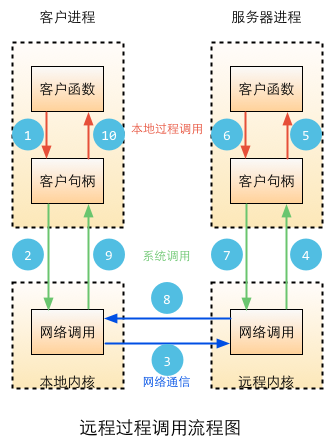
\includegraphics[width=8cm]{8.4.rpc.png}
   \label{図8.8}
   \caption{RPCの動作プロセス図}
\end{figure}

実行時、クライアントマシンがサーバのRPCに対してコールを行うと、そこにはだいたい以下のような10ステップの操作があります:

\begin{enumerate}
  \item クライアントハンドルをコールする。転送引数を実行する。
  \item ローカルシステムのカーネルがネットワーク情報を送信する。
  \item 情報がリモートホストに送信される。
  \item サーバハンドル情報を受け取り、引数を取り出す。
  \item リモートプロセスを実行する。
  \item 実行されたプロセスは結果をサーバハンドルに返す。
  \item サーバハンドルは結果を返し、リモートシステムのカーネルをコールする。
  \item 情報がローカルホストに送信される。
  \item クライアントハンドルがカーネルから情報を取得する。
  \item クライアントはハンドルが返すデータを受け取る。
\end{enumerate}


